\acresetall
\chapter{Testbed Implementation}\label{chapter:implementation}\label{ch:implementation}
This chapter depicts the tools and procedures used in the set up and data preparation prior the machine learning procedures. It includes the steps taken since the start of the work until the moment the first \ac{ML} algorithm started to train. First, an overview of the software and hardware tools is given. Afterwards, a short explanation on the available \ac{ML} libraries and frameworks is presented, along with the reasoning behind their choosing for this work. Lastly, process of measuring the data and preprocessing it is explained in detail, for the data to be ready to be applied to the learning models.
\section{Development Tools}\label{ch:tools}
As stated in the introduction of this thesis, \ac{SDR} and \ac{CR} play an important role in modern communication systems, and is the framework used for most projects at the \ac{CEL}, not only being used as a tool but also being actively contributed to with research results, but also acting as an active agent on open-source improvements. The software and hardware frameworks used are the following:
\subsection{GNURadio}
\begin{figure}[htb]
    \centering
      
\includegraphics[width=0.8\textwidth]{figures/gnuradio_logo}
      \caption{GNURadio logo}
      \label{fig:gnuradio}
\end{figure}
GNURadio \cite{GNURadio2016} is a free and open-source toolkit that provides a large library of signal processing blocks that can be used for several software-defined radio applications. Its functionality does not require a device in the loop, which allows the users to simulate complete communications systems only on a computer. This includes signal sources, modulators and demodulators (such as \ac{PSK} and even \ac{OFDM}), dynamic channel simulators (and virtually any digital filter implementation), math operators, and a plethora of other digital signal processing implementations that have served purposes in academy, research, amateur radio hobbyist and even some government entities. Additionally, thanks to the support for several defined radio hardware \cite{gnuradiohw}, GNURadio grants the capability of transmitting (given the user has a rightful license for this purpose) and receive real signals and process them thoroughly.\\

The usual usage of this software is as follows: the user has a problem or an idea that requires digital signal processing, such as decoding a radio signal or implementing a novel communications' protocol. As said, GNURadio includes several algorithms that serve this purpose, and they are enclosed in so-called blocks. These blocks can then be connected to one another, generating a flow that the signal follows, in a so-called flowgraph, where each block takes a determinate amount of inputs, each input also taking a determinate amount of samples, that undergo the signal processing that the block entitles, and then the block presents its outputs to the next block downstream. If the library provided by GNURadio does not contain implementations that suffice the user needs, new implementations are easily added by the means of a so-called \emph{\ac{OOT}} module, where the user can provide additional applications, and characteristic that makes the scalability of GNURadio a transparent procedure. Lastly, if the user believes that custom implementation can serve a common purpose and other users, the \ac{OOT} can be made public following the open source standards, and this way other users can benefit from the same implementation and probably even contribute to it. An extensive collection of \ac{OOT} that have followed this open source mentality can be found at \ac{CGRAN} \cite{CGRAN}.\\

Regardless of the amount of inputs and outputs on a block, the amount of items required for the algorithm within determines the type of the block:

\begin{itemize}
    \item If for each output produced the block requires only one input item (1:1), then it is a \emph{sync} block.
    \item If the block requires N input items in order to generate 1 output item (N:1), the block is a \emph{decimation} block.
    \item If the block generates M output items for each 1 input item (1:M), the block is a \emph{interpolation} block.
    \item If the block requires to be extended flexibility, requiring N input items for each M output items produced (N:M), the block is a \emph{general} block.
\end{itemize}

Most of the blocks are written in a parametrizable fashion, serving multiple purposes with the same implementation by allowing the user to set different settings which can go from the general point of view, such as the vector length of the signal and its data type, to very specific and detailed parameters such as the taps of a filter or the description of a preamble. \\

The library of algorithms is organized in modules that have a common purpose, and within these modules you find blocks that help achieve that purpose. Examples of such modules are the “gr-qt” module contains the blocks that are intended to be used for visualization purposes using Qt \cite{Qt} and, within this module, blocks such as a “Time sink” and a “Frequency Sink” are found, which are written using Qt and serve as a scope and as a spectrum analyzer, respectively. Another example, more specific, is the gr-channels module, where the user can find different implementations for parametrizable channel simulators, such as fading, frequency selective, and dynamic channel models, among others. Most of these blocks are written in C++ and python, where each block is, in end effect, a class. In the same programming jargon, the module is a namespace. Therefore, the end user is expected to feel comfortable understanding (and, optimally, using-/writing-) these programming languages in order to be able to use these blocks to the fullest. The interconnection of the blocks, i.e. the flowgraph, is written using Python. For the C++ blocks to be available in the Python interface of the flowgraph, this C++ implementation is translated into Python domain by making use of the \emph{\ac{SWIG}}. In addition, multiple blocks can be grouped into a single block that serves a specific purpose, and this is called a hierarchical block.\\

Although coding to the base of the modules and blocks gives the user total control of the details, it is not the only way of getting things done while using GNURadio. The software comes with a \ac{GUI} called \ac{GRC}, which allows the user to drag-and-drop blocks into a canvas and connect them directly with the ease of a click. Even experienced users grab a hold on this \ac{GUI} as it provides ease and versatility along with a visible flowgraph that is easy to understand not only for the user but also to other users whose interest has been drawn to a specific application.\\

Additionally, GNURadio features the \ac{VOLK}\cite{VOLK}, a free librarly of hand-written SIMD mathematical operations used to handle vectorization efficiently. This library is used in this world to optimize operations in the spectrogram generation process, described in section~\ref{ch:spectrogram}.\\

In order to use GNURadio, the recommended installation is done by the means of \ac{PyBOMBS} \cite{PyBOMBS}, which also allows installation of the modules listed at \ac{CGRAN}.

\subsection{Universal Software Radio Peripheral}
\begin{figure}[htb]
    \centering
      
\includegraphics[width=0.5\textwidth]{figures/ettus_logo}
      \caption{Ettus Research's logo}
      \label{fig:ettus}
\end{figure}

One of the \ac{SDR} devices that is supported by GNURadio is the \ac{USRP}, which is developed and produced by the company \emph{Ettus Research\texttrademark} \cite{Ettus}. This company has been a one of the most representative suppliers of \ac{SDR} devices around the globe, and these devices are reknown by its outstanding performance and versatility.\\

During the complete \ac{DySpan} spectrum challenge competition, three different \ac{USRP} devices where used for both \ac{PU} and \ac{SU}. The \ac{PU} used for the transmitter and the receiver the \ac{USRP} X310, which can be seen at Fig.~\ref{fig:x300} \cite{X300}. This device counts with two wide-\ac{BW} \ac{RF} daughterboard slots and a large customizable Xilinx Kintex-7 FPGA. Additionally, it has the capability of using high-speed interfaces such as 10gigE and PCIe, with which a maximmum of 200MS/s full duplex can be travel through the transport link. This \ac{USRP} covers from 10MHz until 6GHz, but based on the daughterboard selected, which serves as \ac{RF} frontend, the frequency of operation of the device can vary.\\

As for the \ac{SU} that was presented by the \ac{KIT} \ac{CEL} group, the transmitter used an \ac{USRP} N210, depicted in Fig~\ref{fig:n210} \cite{N210}. The N210 has a Xilinx Spartan 3A-DSP 3400 FPGA, and can hold up to 100MS/s through a 1gigE link that connects it to a host machine.  This device also requires an \ac{RF} daughterboard as frontend, for which in the \ac{SU} implementation the UBX-40, shown in Fig~\ref{fig:UBX} \cite{UBX}, was used. This daughterboard can operate from 10MHz to 6GHz, providing an instantaneous \ac{BW} of 40MHz. As for the receiver, a B210, shown in Fig~\ref{fig:b210} \cite{B210}, was used. This \ac{USRP} is a fully integrated, two channel device that operates from 70MHz to 6GHz without the need of additional \ac{RF} frontend configuration. It provides Full duplex, MIMO (2 Tx - 2Rx) operation up to 56 MHz of instantaneous \ac{BW}. Furthermore, it counts with a convenient USB 3.0 connection that also serves as power feed.\\

Although this devices provide high-end performance and its versatility is outstanding, \ac{USRP} such as the B210 has still a very competitive price for the quality of its elements. Additionally, Ettus Research\texttrademark is commited with the Open Source community by making its source code available for developers that want to either have a look a it, modify it to add specific functionalities to the \ac{USRP} devices, or contribute to it.

The interface between the devices and the host machine is performed by the \emph{\ac{UHD}}, an open-source software driver provided by Ettus Research\texttrademark that furnish support for all \ac{USRP} devices. This driver supplies API for usage of \ac{USRP} devices as stand-alone, and also provides support for GNURadio via the gr-uhd \ac{OOT}.

\begin{figure}[htb]
    \centering
    \begin{subfigure}[htb]{0.45\textwidth}
        \centering
        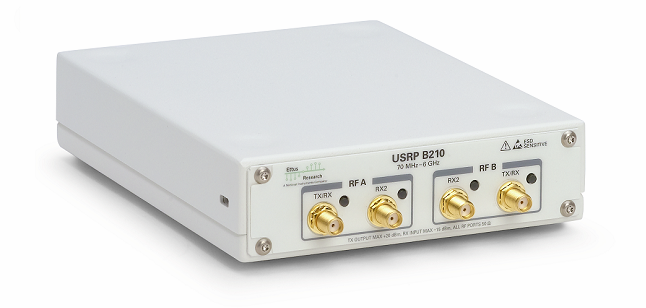
\includegraphics[width=0.7\linewidth]{figures/b210}
        \caption{USRP B210}
        \label{fig:b210}
    \end{subfigure}
    \begin{subfigure}[htb]{0.45\textwidth}
        \centering
        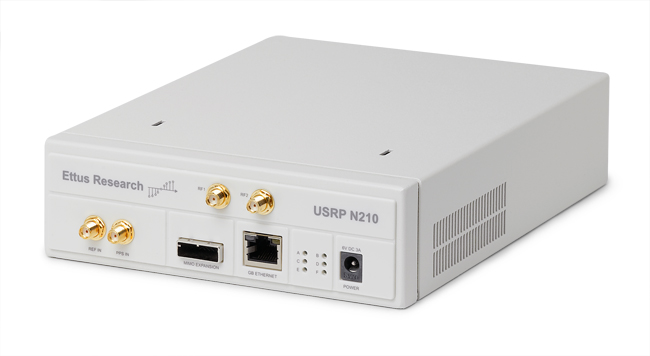
\includegraphics[width=0.7\linewidth]{figures/n210}
        \caption{USRP N210}
        \label{fig:n210}
    \end{subfigure}
    \begin{subfigure}[htb]{0.5\textwidth}
        \centering
        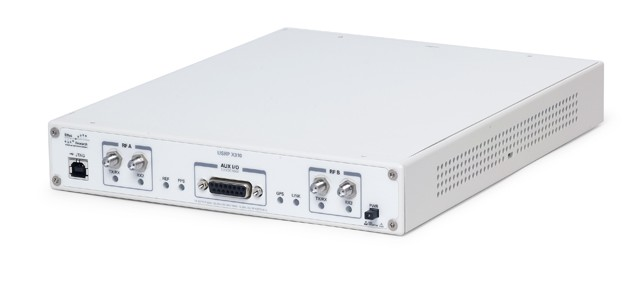
\includegraphics[width=0.7\linewidth]{figures/x310}
        \caption{USRP X300}
        \label{fig:x300}
    \end{subfigure}
    \begin{subfigure}[htb]{0.4\textwidth}
        \centering
        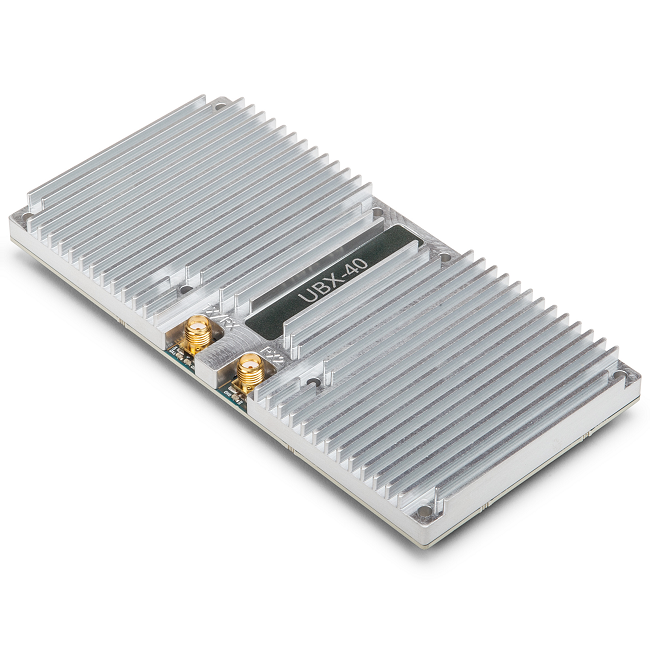
\includegraphics[width=0.6\linewidth]{figures/UBX40}
        \caption{UBX-40 daughterboard}
        \label{fig:UBX}
    \end{subfigure}
    \caption{\ac{USRP} Devices used in the complete DySpan challenge setup}
    \label{fig:ettus}
\end{figure}

For this thesis, the \ac{SU} implementation is reproduced, for which the N210 as transmitter and the B210 as receiver are used.

\section{Machine Learning models in Python and Jupyter}
\begin{figure}[!h]
    \centering
    \begin{subfigure}[htb]{0.45\textwidth}
        \centering
        
\includegraphics[width=\linewidth]{figures/python_logo}
        \label{fig:python}
    \end{subfigure}
    \begin{subfigure}[htb]{0.45\textwidth}
        \centering
        
\includegraphics[width=\linewidth]{figures/jupyter_logo}
        \label{fig:jupyter}
    \end{subfigure}
    \caption{Python and Jupyter logos}
    \label{fig:python_jupyter}
\end{figure}
For the learning part of this work, the focus on the implementation was given to a couple of popular Python libraries that have been effective when dealing with \ac{ML} problems: scikit-learn \cite{SKLEARN} and keras \cite{KERAS}. This libraries were chosen because of the simplicity of their prototyping as well as their effectiveness when providing an implementation that suits the \ac{ML} needs by returning fully trained models with exceptional prediction accuracy, and are described in more detail in the following sections. Additionally, the fact that these libraries are written in Python raises interest because this means that they interface optimally with GNURadio, making the inclussion of these libraries transparent, and having the perks of Python such as easy debugging and extensibility.\\

As for model testing and visualization, Jupyter notebooks \cite{Jupyter} have been used and are presented as part of the code repository of this thesis. What Jupyter provides is an open-source web application in which a number of interpreters for languages such as Python, R, Julia and Scala are embedded, allowing the creation and sharing of interactive register that contains code lines and excecution output along with visualization fields for plots and graphs and documentation in markdown, in what is called \emph{literate programming}. These notebooks can be shared in multiple formats, such as the native notebook format (for further modification of its contents), as well as HTML, \LaTeX{} and PDF (generated with \LaTeX). Moreover, it is nicely integrated with GitHub, so that the notebook can be visualized in the webpage of a remote repository without the need of conversion.\\

Jupyter is the continuation of a long effort for supporting interactive Python interpreters - the IPython Project \cite{IPython}. It has had a bast adoption in the last few years, such that even complete books have been written only using Jupyter as their interface for text editing and code examples. One of the main sources used for this work \cite{Andreas} is one example of such.

\subsection{Scikit-learn}
\begin{figure}[!ht]
    \centering
    
\includegraphics[width=0.4\linewidth]{figures/sklearn_logo}
    \caption{Scikit-learn logo}
    \label{fig:sklearn_logo}
\end{figure}
Scikit-learn, formerly scikits.learn and also known as sklearn, is \ac{ML} library that features an abundance of algorithms for supervised and unsupervised algorithms, including the ones described in section~\ref{ch:ml_algs}. This library came as a result from a \emph{Google Summer of Code} project as a third party extension to SciPy, from where it gets its name. This library was used in this thesis for all the learning based on the extracted features listed in section~\ref{ch:features}.

\subsection{Keras}
\begin{figure}[!ht]
    \centering
    
\includegraphics[width=0.5\linewidth]{figures/keras_logo}
    \caption{Keras logo}
    \label{fig:keras_logo}
\end{figure}
Keras is a high-level neural networks API written in Python that uses TensorFlow \cite{TensorFlow}, CNTK \cite{CNTK} or Theano \cite{Theano} as a backend. The way it is written in a way that allows datascientist to prototype and experiment fast. As per its documentation \cite{KERAS}:\emph{"being able to go from idea to result with the least possible delay is key to doing good research"}, and Keras certainly intends to keep the coding part as simple as possible for the designer to focus on the idea and not the programming of it. For this, it presents and API that is:

\begin{itemize}
    \item User-friendly: with ease for writing, reading and understanding.
    \item Modular: models have a clear begin and end, and they can be easily connected with other models with low to none restrictions.
    \item  Extendible: new functionalities and features are easily added to the mainstream, and the existing codebase is well-documented and exemplified.
\end{itemize}

For this project, Keras is used for convolutional neural networks implementation, using Tensorflow (with GPU support) as a backend.

\section{Setting up development environment}
Identified the tools that are used in this work, now the installation and set up steps are described. This thesis was completely done using Linux-based operative systems, and the steps depicted below have been tested on Fedora 25 as well as on Ubuntu 16.04LTS. Installation in other Linux distributions have small to no difference from these steps. For the setup on a machine using Microsoft Windows\texttrademark, please refer to the documentation of each of the tools listed in section~\ref{ch:tools}.\\

For GNURadio and \ac{UHD}, \ac{PyBOMBS} was used because of the ease it provides on installation, as well as the capability of installing the software in a self contained environment that does not pollute the system domain. However, installation by source can also be performed, and a very detailed sequence of steps can be found in the following for Linux \cite{Linux}, MacOS \cite{OSX} or Windows \cite{Windows}. First of all, \ac{PyBOMBS} needs to be installed, and the recommended way to do so is by using \ac{pip} which, ass well, is the recommended way to install Python packages.  Installation is simply done by running the following command, which will download the latest release:

\begin{lstlisting}
    $ [sudo] pip install PyBOMBS
\end{lstlisting}

In order of install the latest version from git, the following slight modification to that command is needed:

\textbf{NOTE:} along this work only Python2 was used because of compatibility with the current master branch of GNURadio. Future work includes porting this work onto the Py3k improvements of GNURadio, along with newer versions of the following installed libraries.

\begin{lstlisting}[breaklines=true]
    $ [sudo] pip install [--upgrade] git+https://github.com/gnuradio/pybombs.git
\end{lstlisting}

Now, there as option for \ac{PyBOMBS} to parse the best possible configuration specific to the development machine (such as amount of threads used for package installing and a git-cache that speeds up repeatable git clones). This configuration is setup as follows:

\begin{lstlisting}[breaklines=true]
    $ pybombs auto-config
\end{lstlisting}

\ac{PyBOMBS} uses so-called recipes that contain the software description as well as its dependencies. This makes possible to automatically generate dependency trees, that will be automatically installed when a package requires them. The recipes are downloaded nd installed as follows:

\begin{lstlisting}[breaklines=true]
    $ pybombs recipes add-defaults
\end{lstlisting}

Up to this point, \ac{PyBOMBS} has the references necessary to install GNURadio and \ac{UHD}, and it is only needed to specify where in the development machine this software is to be located. For it, we generate a self-contained prefix, which allows us to keep the software all in one place without polluting the system domain. The next command creates the directory {\raise.17ex\hbox{$\scriptstyle\sim$}}\textbackslash workarea, gives it the alias "workarea" (which will help \ac{PyBOMBS} identify this prefix uniquely), and will start the GNURadio installation after installing all its dependencies, \ac{UHD} included:

\begin{lstlisting}[breaklines=true]
    $ pybombs prefix init ~/workarea -a workarea -R gnuradio-default
\end{lstlisting}


In order to install the \ac{ML} libraries, there are multiple options as well. The libraries can be installed using pip with the following command:

\begin{lstlisting}[breaklines=true]
    $ [sudo] pip install numpy scipy pandas graphviz jupyter scikit-learn tensorflow keras
\end{lstlisting}

Numpy and Scipy should have been installed during the GNURadio installation, but are listed in the command for completeness' sake. It is also recommended to install this tools in a dedicated Python Environment, such as Conda or Virtualenv. Procedures on how to generate these virtual environments, and already saved environments that can be pulled and installed (included the versions used in this work) are included in the GitHub repository of this thesis \cite{repo:cognitive_radio_ml}.

\textbf{NOTE:} For training using Keras/Tensorflow, and given that the development machine has a compatible graphic card, it is recommended to install Tensorflow with GPU support. By doing so, the training times are reduced drastically. This work was developed and written using a Lenovo Thinkpad W541, which counts with a NVIDIA Quadro K2100M Graphic card, compatible with CUDA. For this dedicated installation, a combined procedure from \cite{Yadak} and \cite{Andrews} was used.

\section{Data set Generation}
This part of the work regards the steps taken in order to have the data ready for the \ac{ML} algorithms to learn from it. It covers the testbed setup, the raw data (I/Q samples) measurement, and the data preprocessing.
\subsection{Measure Campaign}\label{ch:measure}
The first step taken was to set up the \ac{PU} communication link over the air, and recording the raw samples just as the \ac{SU} would be able to "hear" them. The measurement setup is shown in Fig~\ref{fig:measurement}, where two parts are labeled separately.

\begin{figure}[!htb]
    \centering
    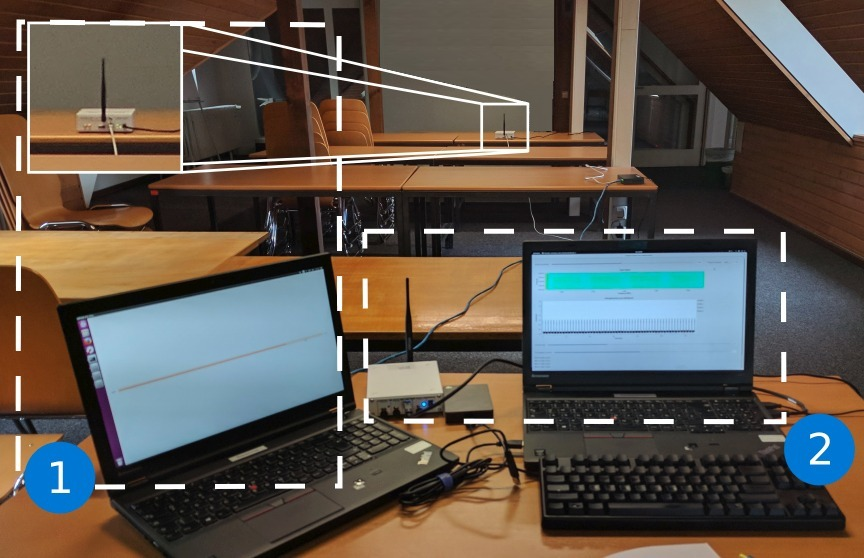
\includegraphics[width=0.5\linewidth]{figures/mod}
    \caption{Measurement Setup}
    \label{fig:measurement}
\end{figure}

The part labeled with \raisebox{.5pt}{\textcircled{\raisebox{-0.9pt} {1}}} regards the transmission part, which is going to be sending frames over the air in ten different fashions, described in Table~\ref{table:scenarios}.  The host machine in this part has the connection to the database, from where the information frames are extracted and put as payload of the transmitted frames. Additionally, the GNURadio flowgraph that generates the signal, which can be seen in Fig~\ref{fig:PU_flowgraph}, is also hosted and run from this computer. A summary of the path that a frame travels from the database until the transmitter is as follows: in Fig.~\ref{fig:PU_flowgraph} it can be seen that a connection to the database is done in the "Cmd pktgen" block, which is in charge of retreiving the information frames from the database, in form of \ac{PDU}, and feeding them into the signal processing blocks. After converting the \ac{PDU} into a byte tagged stream (a stream of data that has metadata attached to it in form of tags), the stream flows into the \ac{OFDM} transmitter block, which is a hierarchical block that allocates the carriers for an \ac{OFDM} transmission, applies a \ac{FFT} to them, and appends a cyclic prefix.

Right after, the output, which is a complex I/Q tagged stream, is then converted again into \ac{PDU} and feed into the packet controller block. This block is in charge of generating the different scenarios that are set to be identified in this thesis by the means of learning techniques. The parameters of this block are not modified along this work, except one: the "scenarios list". By setting the scenario list to an specific value from 0 to 9, a determinate behavior can be set and recorded, and when this samples (after the feature extraction of section~\ref{ch:features} are paired to the selected scenario, they have the form (input, output), suitable for supervised learning techniques. The rest of the flowgraph, consistent of resampling and multiplying with a sine signal, corresponds to a traditional mixing to the specific channels between the 10MHz \ac{BW} centered at 3.195GHz. As for the \ac{RF} frontend, a N210 \ac{USRP} was used, which in the flowgraph is represented as the "UHD:USRP sink" block.

\begin{figure}[!htb]
    \centering
    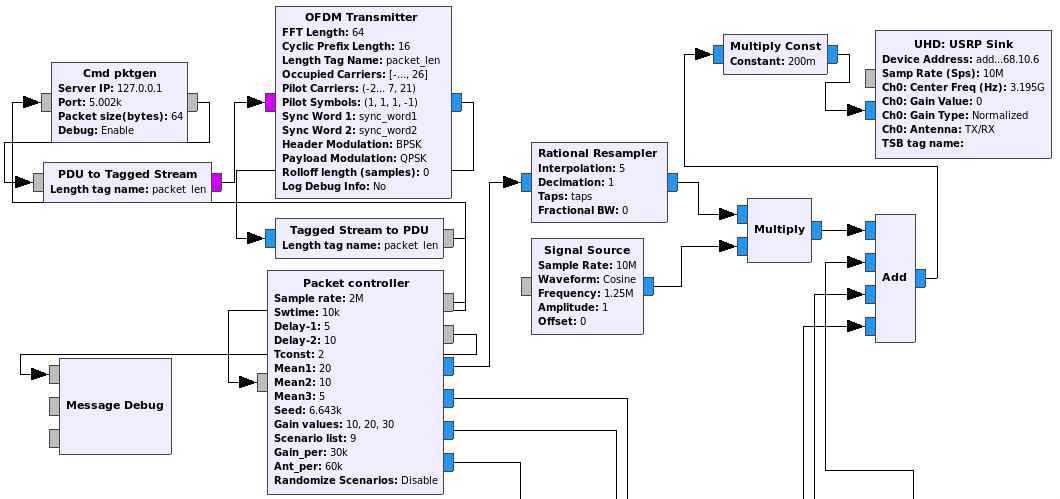
\includegraphics[width=\textwidth]{figures/PU_flowgraph}
    \caption{\ac{PU} GNURadio flowgraph}
    \label{fig:PU_flowgraph}
\end{figure}

The part of the Fig~\ref{fig:measurement} labeled with  \raisebox{.5pt}{\textcircled{\raisebox{-0.9pt} {2}}}  corresponds to the recording system. In this machine, a very simple flowgraph has been implemented and is shown in Fig~\ref{fig:recording_flowgraph}. An "UHD: USRP source" block, which in real life is an \ac{USRP} B210, is connected directly to a couple of scopes: A Waterfall sink and a Time Sink. These scopes, however, are only used for supervision of the presence of energy over the air, and have no effect whatsoever on the recorded signal. The main path is then the "File sink", which directly saves the data presented at is input into a file, and the "Head block" which serves as gauge to limit the amount of data that is saved to disk. Taking disk space into consideration, it was decided to record 1 minute of raw samples per scenario: 30 seconds with the presence of DC offset in the transmitter, 30 seconds without it. The DC offset is taken into consideration because the assumption is made that there is no strict control on how the \ac{PU} transmissioin is made appart from the specs given, so this is an attempt to cover every possible situation. The reason behind this time limitation is the amount of data that has to be taken into consideration. The math behind it is as follows:
\begin{equation}
    \frac{\SI{10}{\mega S}}{\SI{1}{s}} \cdot \SI{60}{s} \cdot \frac{\SI{8}{\byte}}{\SI{1}{S}} = \SI{4.8}{\giga\byte}
\end{equation}

\begin{figure}[!htb]
    \centering
    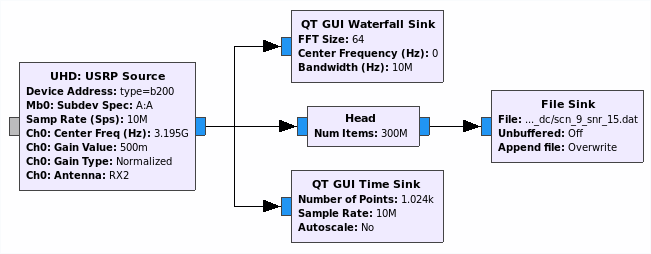
\includegraphics[width=\textwidth]{figures/recording_flowgraph}
    \caption{Flowgraph used to record over-the-air samples}
    \label{fig:recording_flowgraph}
\end{figure}

Each sample is complex valued of 64 bits, having 32-bit for the real part and 32-bit for the imaginary part, totalling \SI{8}{\byte} per sample. At a rate of 10MSps used at the DySpan Spectrum Challenge, a minute of measurement corresponds to \SI{4.8}{\giga\byte} of data. Now, it is of interest to have measurements of different \ac{PU} signal power, in order to determine the performance of the learning algorithms facing low \ac{SNR}. It was determined that measurements for \ac{SNR} values equals to \SI{-5}{\decibel}, \SI{-2.5}{\decibel}, \SI{0}{\decibel}, \SI{2.5}{\decibel}, \SI{5}{\decibel}, \SI{10}{\decibel}, \SI{15}{\decibel} would represent the overall performance of the algorithm facing bad \ac{SNR} as well as "good-enough" \ac{SNR}. This means that the measurement was repeated 7 times per scenario.

\begin{equation}
    \SI{4.8}{\giga\byte} \cdot 7 \text{ SNR levels} \cdot 10 \text{ scenarios} = \SI{336}{\giga\byte}
\end{equation}

This clearly represents a limitation for the host machine of the lab, that has shared resources with other users and, regardless and in total, has only a total of \SI{500}{GB} of hard disk. However, this is done this way as an attempt to reproduce the challenge setup closely. Clearly, other methodologies could have been followed, and a short argument regarding this detail is given in chapter~\ref{ch:conclusions}.

Here is important to state a remark on how the \ac{SNR} was calculated, and how the control over it was applied to ensure that the samples are independent and that they contain the right information. First, a calibration procedure was made on the \ac{PU} transmitter, using a handheld spectrum analyzer. Starting with the maximum gain on the transmission chain on the N210, it was double checked that by reducing a value XdB on the gain, a decrease of XdB in the power measurement was also seen. An example for this is shown in Fig~\ref{fig:snr_spec}, where a variation of 5dB gain is applied at the transmitter. Additionally, the average received power was also plotted at the receiver side, along with SNR calculations shown in the GUI as labels, as seen in Fig~\ref{fig:snr_receiv}.

\begin{figure}[!htb]
    \centering
    \begin{subfigure}[htb]{0.45\textwidth}
        \centering
        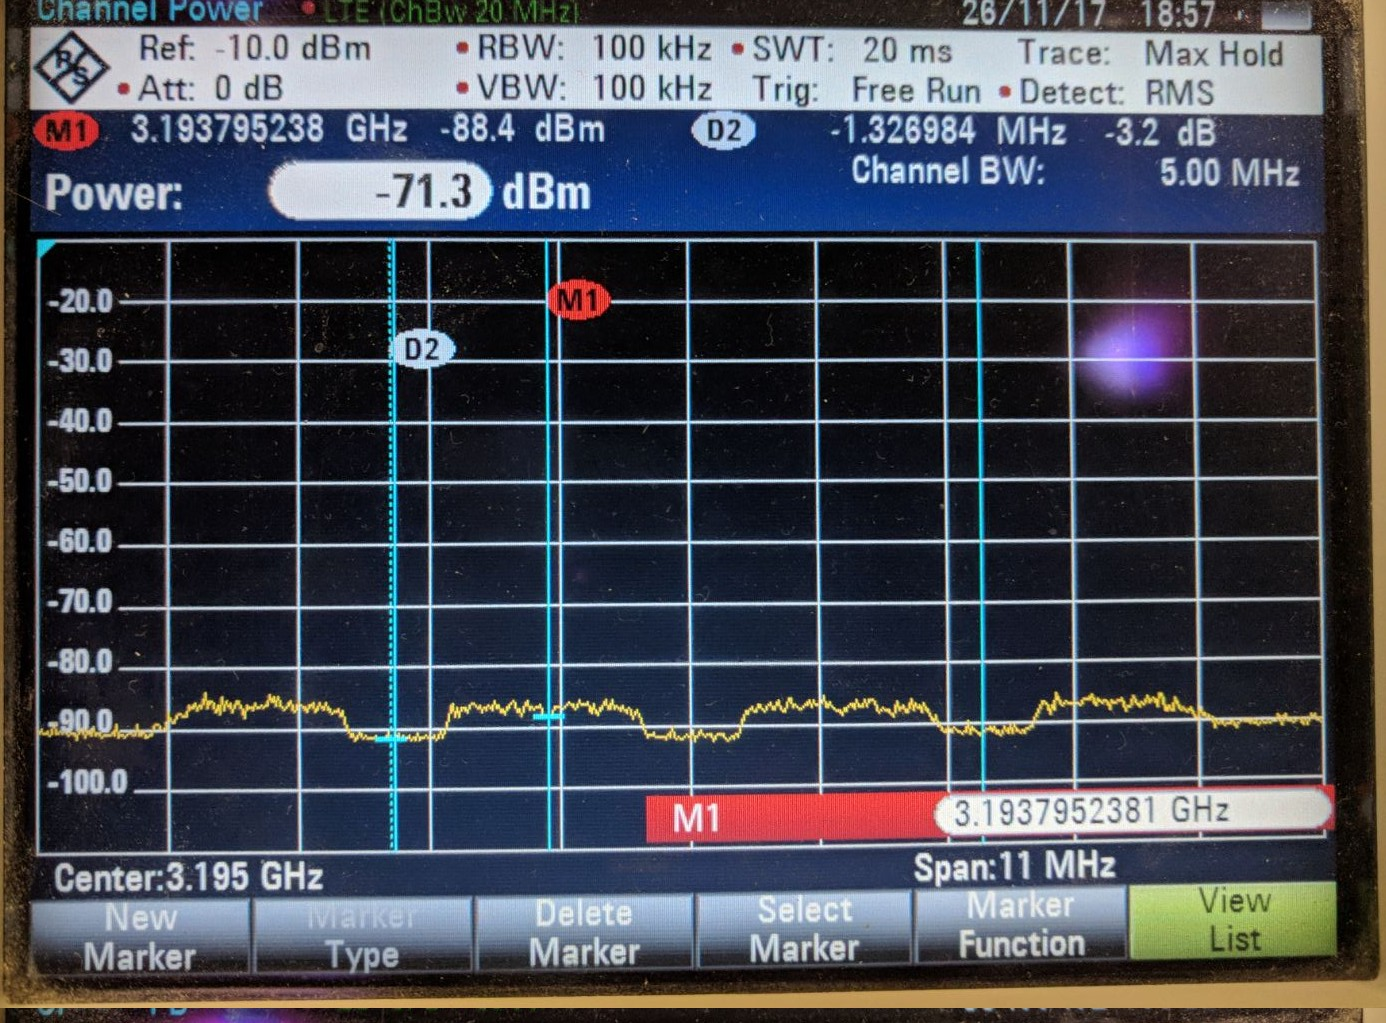
\includegraphics[width=\linewidth]{figures/snr_spec_5}
    \end{subfigure}
    \begin{subfigure}[htb]{0.45\textwidth}
        \centering
        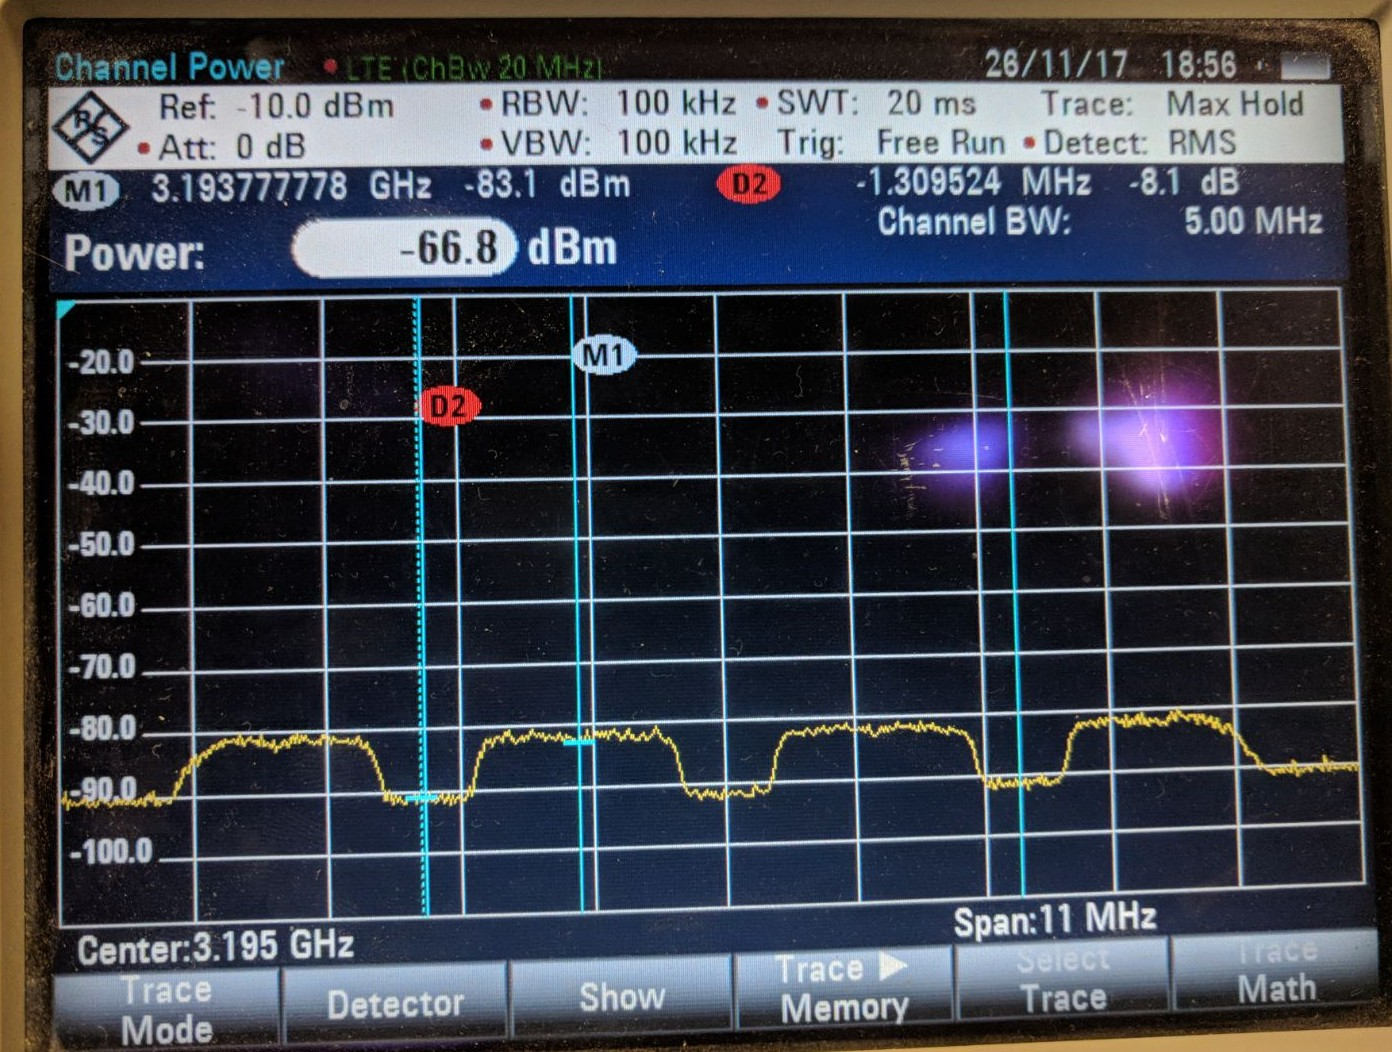
\includegraphics[width=\linewidth]{figures/snr_spec_10}
    \end{subfigure}
    \caption{Calibration of gain variation on PU transmitter (5dB variation)}
    \label{fig:snr_spec}
\end{figure}

\begin{figure}[!htb]
    \centering
    \begin{subfigure}[htb]{0.45\textwidth}
        \centering
        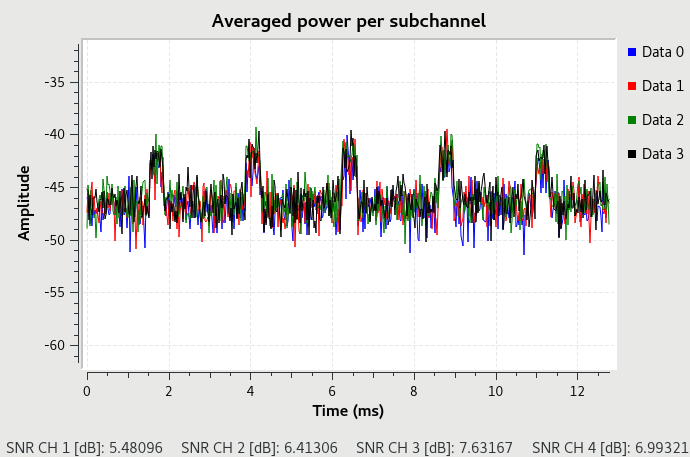
\includegraphics[width=\linewidth]{figures/snr_receiv_5}
        \caption{SNR={\raise.17ex\hbox{$\scriptstyle\sim$}}5dB}
    \end{subfigure}
    \begin{subfigure}[htb]{0.45\textwidth}
        \centering
        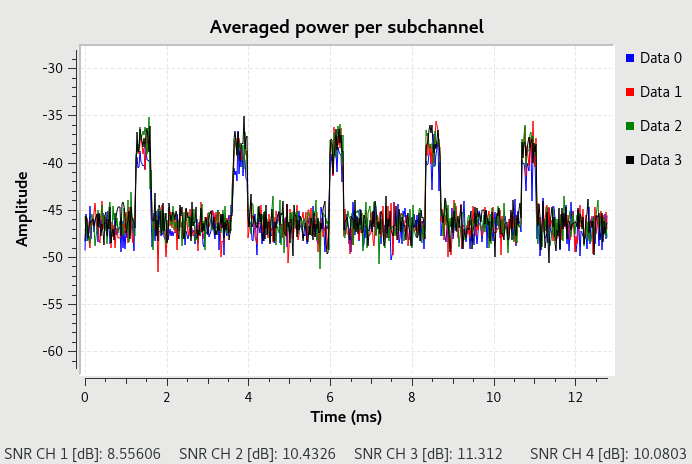
\includegraphics[width=\linewidth]{figures/snr_receiv_10}
        \caption{SNR={\raise.17ex\hbox{$\scriptstyle\sim$}}10dB}
    \end{subfigure}
    \caption{SNR display at receive side}
    \label{fig:snr_receiv}
\end{figure}

\subsection{Feature Engineering}\label{ch:features}
Having recorded the raw I/Q samples, it is required to apply signal processing techniques in order to extract features that this data could entitle and that would be representative to identify the scenario that the \ac{PU} transmission is describing. For this, the implementation that was used in \cite{Wunsch2017} was used. The flowgraph that serves the purpose of feature extraction is shown in the Fig~\ref{fig:feature_extraction}. In Fig~\ref{fig:ed}, the files recorded from the \ac{PU} transmission are passed through an \ac{FFT}, and then the "Energy Detection" block is in charge of determining which channel has an measure of energy greater than the given threshold, which can be set as a block parameter. This block has 8 outputs: the top four provide the average power per subchannel, useful for plotting. Fig.\ref{fig:snr_receiv} was plotted using these outputs; the bottom four send simply ones when the channel is identified as occupied, and zeros if the channel is identified as free.

\begin{figure}[!htb]
    \centering
    \begin{subfigure}[htb]{\textwidth}
        \centering
        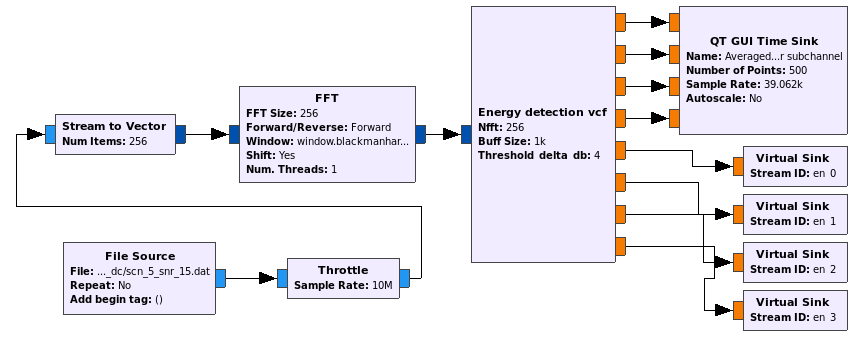
\includegraphics[width=\linewidth]{figures/feature_extraction_1}
        \caption{Energy Detection}
        \label{fig:ed}
    \end{subfigure}
    \begin{subfigure}[htb]{\textwidth}
        \centering
        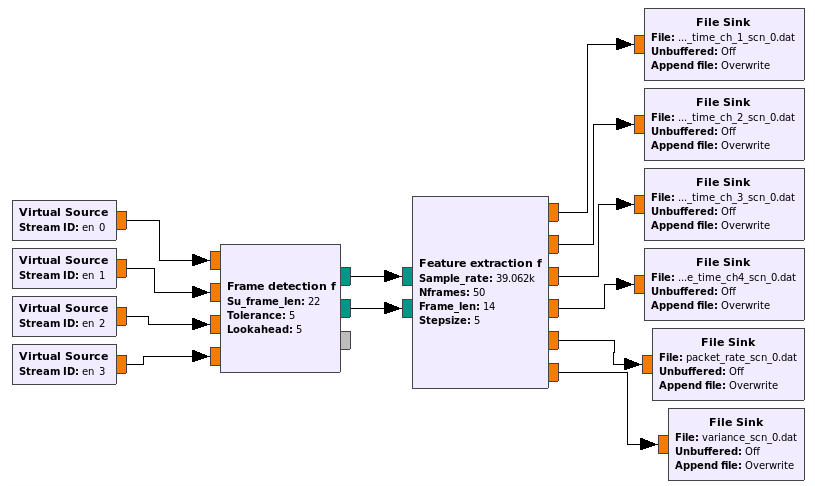
\includegraphics[width=\linewidth]{figures/feature_extraction_2}
        \caption{Frame Events detection and write features to file}
        \label{fig:frame_events}
    \end{subfigure}
    \caption{GNURadio Flowgraph for feature extraction}
    \label{fig:feature_extraction}
\end{figure}

The second part of the flowgraph, shown in Fig~\ref{fig:frame_events} uses the boolean-like output from the "energy detection" block and analyzes them as \emph{frame events}, identifying the frames over the air and cathegorizing them as \ac{PU} frames or \ac{SU} frames based on its length, and generating these frame events if the analyzed frame per channel corresponds to the \ac{PU}.  Then, these events are taken at the "Feature Extraction" block, which generates three main features based on its inputs:

\begin{itemize}
    \item the average interframe time, i.e. the time delay between \ac{PU} frames.
    \item the packet rate, meaning the amount of packets/frames that are passing through per second.
    \item the variance of the interframe time, which intends to determine if this interframe time is deterministic or stochastic and, if the later, with which variation.
\end{itemize}

Although these are effectively only three features, the interframe time is analyzed per channel, which explains the 6 outputs of the "feature extraction" block. This information is then written to disk in different files. This procedure is repeated for all the files saved during the process described in section ~\ref{ch:measure}, generating a total of:

\begin{equation}
    \text{10 scenarios} \cdot \text{ 7 SNR levels } \cdot \text{6 feature files } = \text{ 420 files }
\end{equation}

This files are provided in the final Dataset product of this work, and a convenient script that automates the process of the feature extraction is provided at \cite{repo:cognitive_radio_ml}. As stated at the beginning of the chapter, this features will be used for supervised learning, and the results are recorded in chapter~\ref{ch:evaluation}

\subsection{Spectrograms generation}\label{ch:spectrogram}

The feature extraction process is convenient and works outstandingly as seen in \cite{Wunsch2017}. However, it depends on a good \ac{PU} power level in order for the frame events to be generated. A way to go around this limitation is applying a different technology, such as image recognition using \ac{ConvNet}. The idea is to generate images that describe the unique characteristics of each scenario, and feed them to an image classificator. The images that better suit this need are the spectrograms. Based on the work of \cite{Paisana2017}, spectrograms were generated using the GNURadio flowgraph shown in Fig~\ref{fig:specgram_generation}

\begin{figure}[!htb]
    \centering
    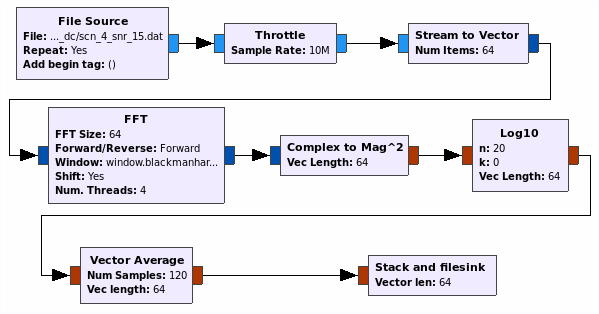
\includegraphics[width=\textwidth]{figures/specgram_generation}
    \caption{GNURadio Flowgraph for spectrogram generation}
    \label{fig:specgram_generation}
\end{figure}

Most of the procedure is rather straight forward: the I/Q data files are read and its stream is moved into a vector for the \ac{FFT} calculation. Our target images are going to have a 64x64 pixels dimension, so that sets as well the FFT size to 64. The following blocks calculate the power of the signal. The last two blocks require a more detailed explanation.
The "Vector average" block calculates the arithmetic mean over a certain amount of vectors, as seen in Fig~\ref{fig:vectoravg}. For the sake of clarity, it can be assumed that this block operates over a matrix (or a 2-dimensional array) of dimensions NxM, being M the length of the input vectors, set in the block via the parameter "vector length" and set to 64 in this specific case, and N the amount of vectors to operate, set in the block via the parameter "Num Samples" and set to 120, which will become clear shortly.\\

\begin{figure}[!htb]
    \centering
    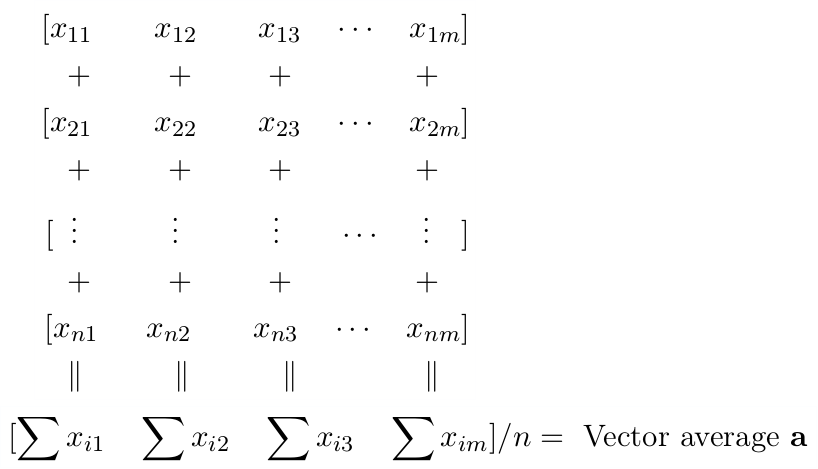
\includegraphics[width=0.7\textwidth]{figures/vectoravg}
    \caption{Operations made in "Vector Average" block}
    \label{fig:vectoravg}
\end{figure}

%\begin{align*}
    %[x_{11}\quad \quad x_{12} \quad \quad x_{13}\quad \cdots\quad x_{1m}] \\
       %+   \qquad \;  + \qquad \; +  \quad \quad \quad \quad + \quad     \\
    %[x_{21}\quad \quad x_{22} \quad \quad x_{23}\quad \cdots\quad x_{2m}] \\
       %+   \qquad \;  + \qquad \; +  \quad \quad \quad \quad + \quad     \\
    %[\; \; \vdots \qquad \quad \vdots \qquad \quad \vdots \quad  \; \; \; \cdots \quad \; \vdots \quad] \\
       %+   \qquad \;  + \qquad \; +  \quad \quad \quad \quad + \quad     \\
    %[x_{n1} \quad \; \; x_{n2} \qquad x_{n3}\quad \cdots\quad x_{nm}] \\
    %\; \; \; \parallel \qquad \quad \parallel \qquad \quad \parallel \quad  \; \; \;  \qquad \; \parallel \quad \\
%\end{align*}
%\[
    %[\sum{x_{i1}} \quad \sum{x_{i2}} \quad \sum{x_{i3}} \quad \sum{x_{im}}] / n = \text{ Vector average }\mathbf{a}
%\]
%\[
%\begin{bmatrix}
    %a_{11} & a_{12} & a_{13} & \dots  & a_{1m} \\
    %a_{21} & a_{22} & a_{23} & \dots  & a_{2m} \\
    %\vdots & \vdots & \vdots & \ddots & \vdots \\
    %a_{m1} & a_{m2} & a_{m3} & \dots  & a_{mm}
%\end{bmatrix}
%\]
%\begin{align*}
    %[a_{11}\quad \quad a_{12} \quad \quad a_{13}\quad \cdots\quad a_{1m}] \\
    %[a_{21}\quad \quad a_{22} \quad \quad a_{23}\quad \cdots\quad a_{2m}] \\
    %[\; \; \vdots \qquad \;\;\; \vdots \qquad \quad \vdots \quad  \; \; \; \cdots \quad \; \vdots \quad] \\
    %[a_{m1} \; \quad a_{m2} \qquad a_{m3} \;\;\;  \cdots \;\; a_{mm}] \\
%\end{align*}

\begin{figure}[!htb]
    \centering
    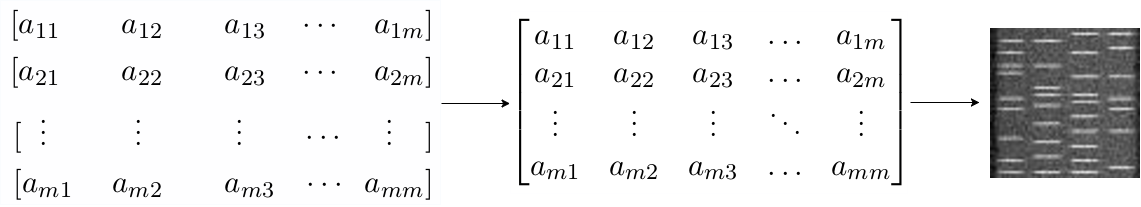
\includegraphics[width=\textwidth]{figures/stack_n_save}
    \caption{Operations made in "Stack and Filesing" block}
    \label{fig:stacknsave}
\end{figure}

The block takes 120 vectors and presents at its output the arithmetic mean according to the matrix. After that, the block "Stack and filesink" takes 64 averaged vectors, stacks them vertically and generates an image object that is later saved as a JPEG image to disk, as seen in Fig~\ref:fig{stacknsave}. These images are then used for the image classification. From the files recorded using the procedure described at section~\ref{ch:measure}, a total of 84700 pictures is generated, from which 90\% is used for training the \ac{ConvNet} and 10\% is used as testing set.

